\section{Evaluation}

In this section we will present an evaluation of our framework using simulation and a prototype implementation. We use QualNet~\cite{16} with a sensor networks plug-in for simulations. Each simulation run takes 15 minutes. The reported workloads ($\lambda$ or $l$ in figures) are the number of requests per second for the whole network. A node is selected uniformly as a destination of each request. Prototype results are averaged over 1000 requests. Reported results are for end-to-end delay of requests from front-end to end-node unless mentioned otherwise. Parts used for our prototype are over-viewed in Section~\ref{sec:background}. The evaluation will start with analyzing the behavior of service times. Then, delay time measurements are displayed and compared with the model. After that, we show results for the prototype implementation. Finally, we will explore the efficacy of using the model to maximize sleeping times while maintaining an average delay.

\subsection{Service time}
In this section we will investigate the service time, mentioned in section~\ref{sec:model}. We will observe two topologies with one and two end-nodes. In each experiment, we will plot the average service time while varying the sleep time for different workloads. The calculated service time is obtained by rearranging Equation~\ref{eq:waiting_2} and solving for it by substituting the remaining known variables. We make an assumption that the distribution of service times is discrete; results in next subsections support that this is a working approximation. 

\begin{figure}[t]
\centering
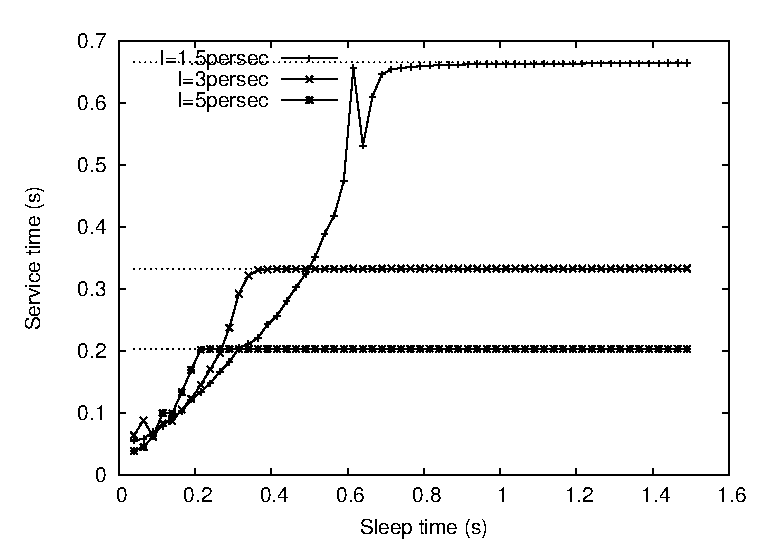
\includegraphics[scale=0.65]{figures/3node_varySleep_sim_x.eps}
\caption{Service time as calculated from the model given the results of a three-node network simulation}
\label{fig:3nodes_x}
\end{figure}

\begin{figure}[t]
\centering
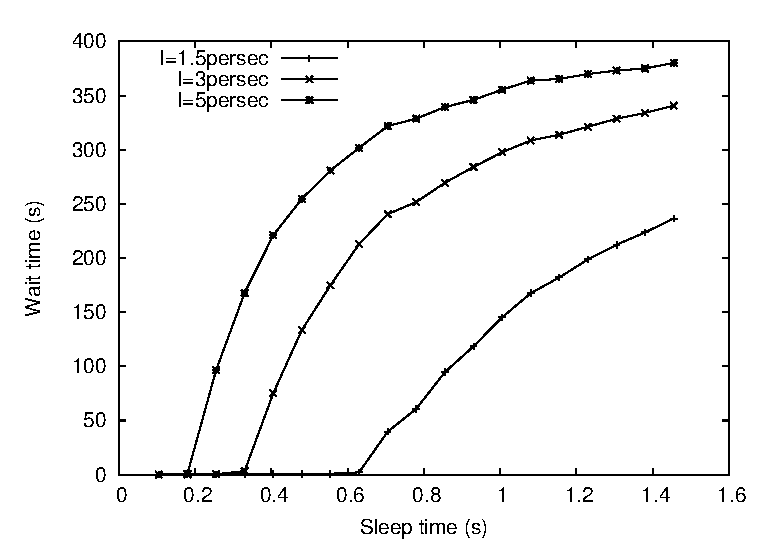
\includegraphics[scale=0.65]{figures/3node_varySleep_sim_large.eps}
\caption{Wait times of a three-node network}
\label{fig:3nodes_large}
\end{figure}

\begin{figure}[t]
\centering
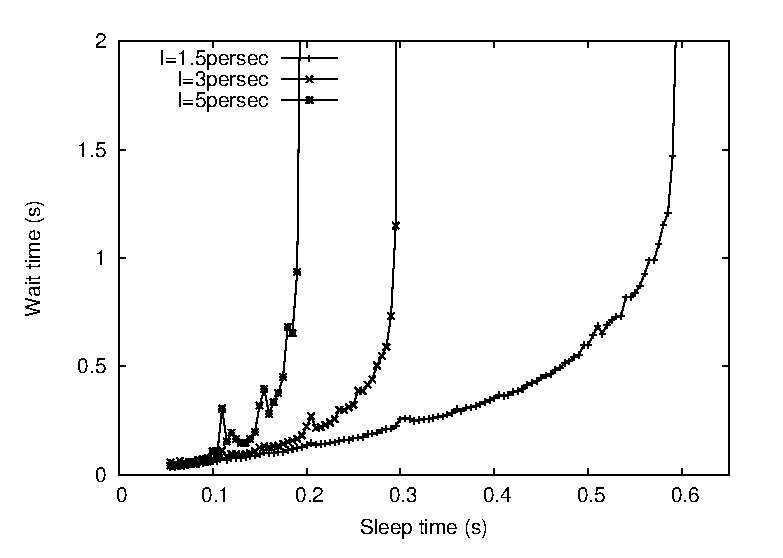
\includegraphics[scale=0.65]{figures/3node_varySleep_sim_small.eps}
\caption{Wait times of a three-node network focusing on non-saturated channel values}
\label{fig:3nodes_small}
\end{figure}

In Figure~\ref{fig:3nodes_x} the service times of a topology with three end-nodes are displayed while varying sleeping times. The figure shows results for three different workloads. It is clear from the figure that the service time is upper bounded. The interesting observation is that this upper bound is equal to the inverse of the workload, \emph{i.e.}, the average inter-arrival time. This confirms our hypothesis since the intensity of the system is not allowed to exceed a value of one. We call the point where the service time converges as the \emph{saturation point}. Prior to the saturation point, the service time increases proportionally to sleep time and workload. This observation can help us in using our model; for sleeping times smaller than the saturation point we set the value for the service time according to an approximation of a monotonic function. We use a linear approximation that will guarantee an upper bound of service time. Otherwise, sleeping time is set to be approaching the average inter-arrival time.

Another observation is that although the service time values are increasing prior to saturation, their effect is less observable until the intensity is approaching 1. This is due the dominance of the second term in equation~\ref{eq:waiting_2} that corresponds to (\emph{sleeping time}). This is demonstrated in Figures~\ref{fig:3nodes_large} and \ref{fig:3nodes_small}. Prior to the saturation point, the wait times are relatively small and dominated by the sleeping time, as shown in Figure~\ref{fig:3nodes_small}. However, after the saturation point, Figure~\ref{fig:3nodes_large}, the intensity is approaching 1 and therefore causes a dramatic increase in wait times.

\begin{figure}[t]
\centering
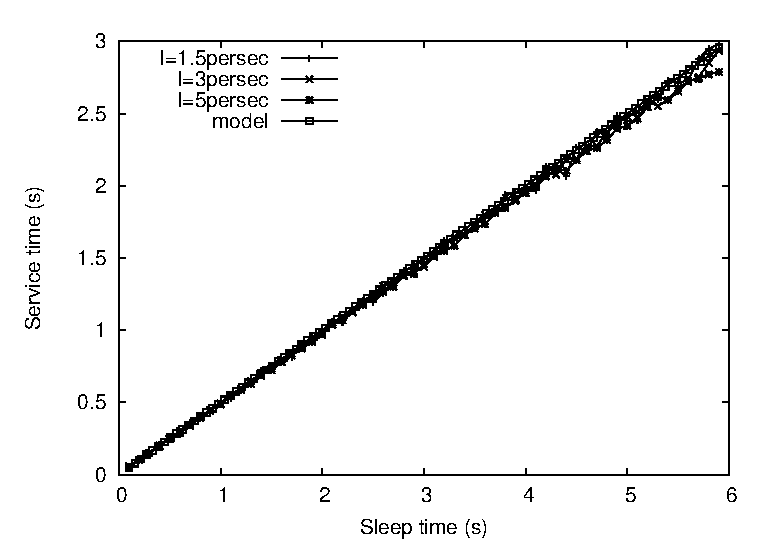
\includegraphics[scale=0.65]{figures/1node_varySleep_sim.eps}
\caption{Sleep times for a network with one end-node compared with the model}
\label{fig:1node}
\end{figure}

\begin{figure}[t]
\centering
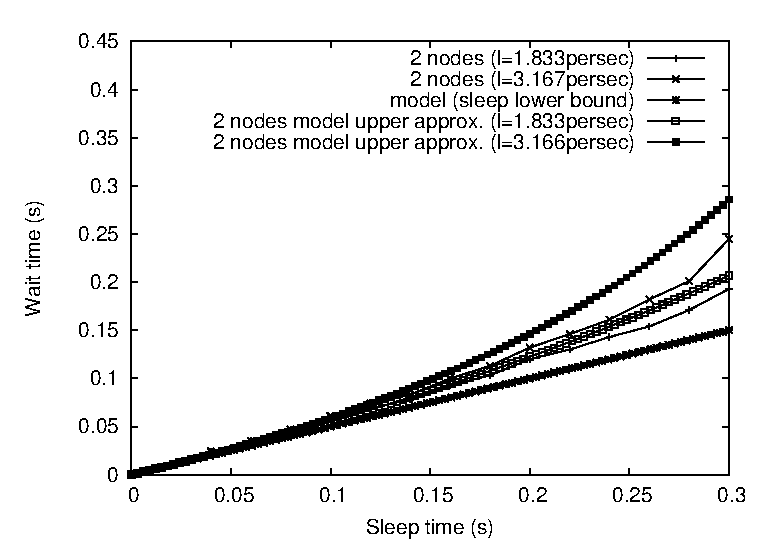
\includegraphics[scale=0.65]{figures/sleep_model_2nodes.eps}
\caption{Comparing wait times for a 2-node network with upper and lower bounds obtained through model}
\label{fig:wait_times_2nodes}
\end{figure}


\subsection{Model validation}
In this section we will demonstrate the behavior of 1 and 2 end-nodes scenarios. We first observe how a small value of service time can make the wait time derivable from the sleeping time only. First, we show a baseline case for a topology with one end-node in Figure~\ref{fig:1node}. In this scenario, the channel does not saturate and the service times are always small, rendering wait times to be dominated by sleep times. Therefore, the difference in workloads is not observed and all plots overlap with the model. Now, we show a scenario with two end-nodes and show how the model predicts behavior when sleep times approaches saturation point. Figure~\ref{fig:wait_times_2nodes} shows these results. Two runs with different workloads are shown. A lower bound is the delay experienced by the sleep cycle and is experienced regardless of workload. An upper bound is calculated using our approximation. We observe that as the number of nodes or amount of workload is increasing, the approximation becomes more conservative.

\begin{figure}[t]
\centering
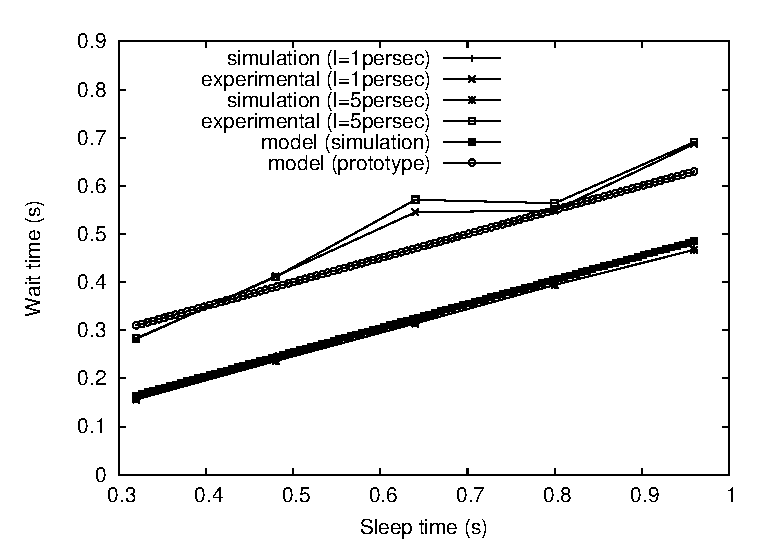
\includegraphics[scale=0.65]{figures/1node_both.eps}
\caption{Comparing wait times of simulation, prototype, and model for a single node network}
\label{fig:1node_both}
\end{figure}

\begin{figure}[t]
\centering
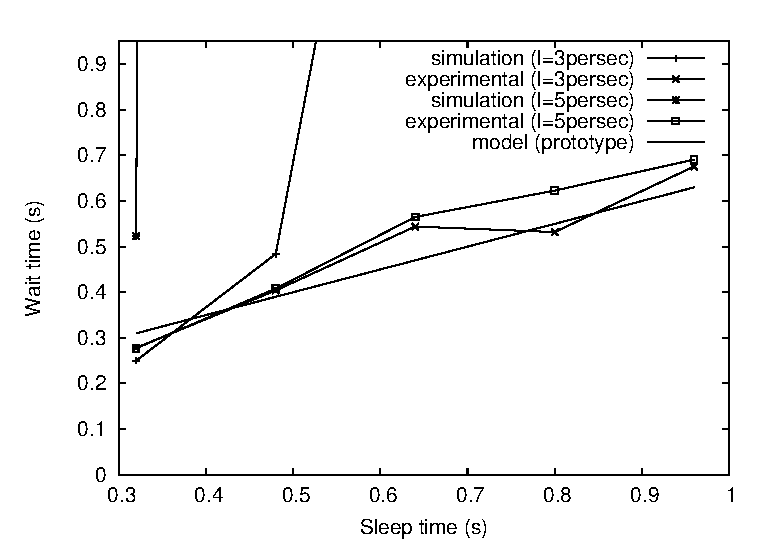
\includegraphics[scale=0.65]{figures/2node_both.eps}
\caption{Comparing wait times of simulation, prototype, and model for a two-node network}
\label{fig:2node_both}
\end{figure}


\subsection{Prototype Evaluation}
Now we will display results obtained from our model to demonstrate its behavior in accordance to our model. In Figure~\ref{fig:1node_both} the results of a single-node prototype is compared to simulation and model. Results shown for the prototype are of the RTT due to difficulty in measuring end-to-end request delay. The same behavior is experienced by both node. However, Since we include the whole RTT for the prototype the effect of end-node transmission and processing is accounted, which is approximated to be equal to 0.1 seconds. Next, we present results for a two-node network in Figure~\ref{fig:2node_both}. It is observed that the prototype acts similarly to the single-node network case, hence saturation is not achieved. However, the simulation saturated and values became much larger than the expected non-saturated case. This demonstrated the effect of channel and physical condition on the saturation point. We were not able to test for larger number of nodes in our prototype due to the lack of hardware. We however, showed that our findings for the saturated case are observed in the prototype.

\begin{figure}[t]
\centering
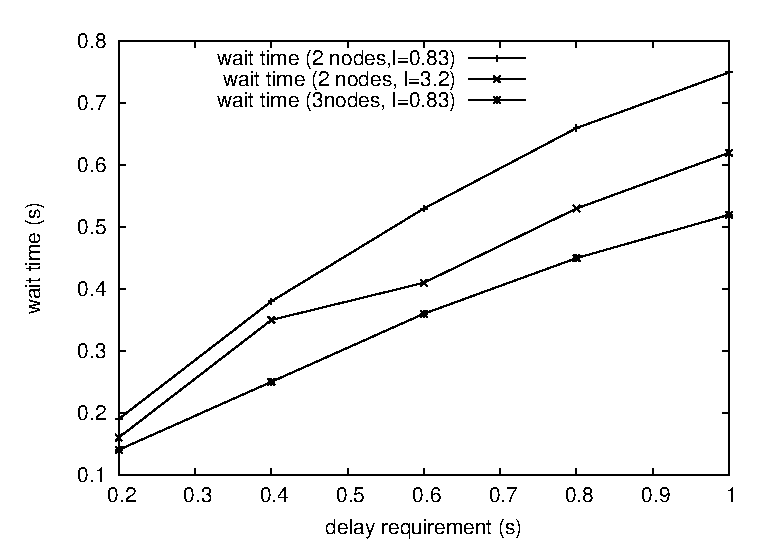
\includegraphics[scale=0.65]{figures/test_2nodes.eps}
\caption{assigning sleep times to achieve an upper bound on wait times for networks with 2 and 3 nodes}
\label{fig:test_2nodes}
\end{figure}

\subsection{Assigning sleeping times}
In this section we will put our findings to the test. For three networks with 2, 3 and 10 nodes respectively, we will calculate sleeping times that guarantee an upper bound for delay. Results are shown in Figure~\ref{fig:test_2nodes}. Having a larger number of nodes or a larger workload make the approximation more conservative, as shown in the figure. Furthermore, a larger requirement make the calculated sleeping time more conservative relatively. This is due approaching saturation which makes the calculation of wait times more sensitive to service times.



